%-------------------------------------------------------------------------------
% File: specifications.tex
%
% Author: Marco Pinna
%         Created on 08/04/2022
%-------------------------------------------------------------------------------
\chapter*{Specifications}
In what follows, the design and implementation of a CRC algorithm on a Xilinx Zynq Board is carried out.\\
The specifications are the following (translated from Italian):
\hfill \break
\begin{displayquote}
    \begin{specifications}
    {\Large Implementation of a CRC algorithm}\\
		Design a digital circuit that implements the Cyclic Redundancy Check (CRC) algorithm, both for the \textit{sender} and for the \textit{receiver}, according to the specifications below.
		Such algorithm is a powerful control method that exploits the idea of redundancy; a sequence of F redundant bits (Frame Control Sequence FCS)is added (by the sender) to a data sequence M, so that the transmitted message, on M+F bit, is divisible by a predefined divisor called CRC polynomial. The receiver, through a division by the same polynomial used by the sender, can detect the correctness of the received data.\\
\\
	Message M=56 bits\\
	Frame Control Sequence F=8 bits\\
	CRC polynomial of degree 9: $x^{8} + x^{4} + x^3 + x^{2} + 1$\\
	(The binary representation of the polynomial will therefore be 100011101)\\
	Transmitted message M+F=64 bit
	
		
		
		\begin{figure}[H]
		    \begin{center}
	        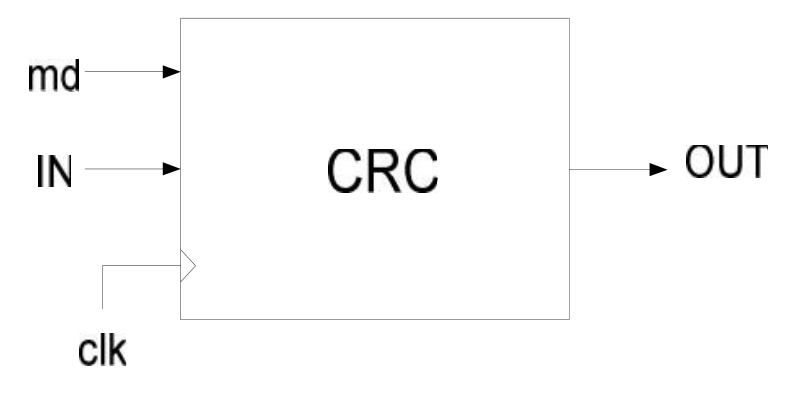
\includegraphics[scale=0.5]{img/high_lvl_schematics.png}

        	\label{fig:high_lvl_schematics}
    		\end{center}
    	\vspace*{-0.4cm}
\end{figure}

Through the \texttt{md} signal one can set whether the circuit is to be used as sender or as receiver.\\
When operating as receiver the last F values of OUT indicate the correctness of the received message.\\
\\
\\
\underline{The final project report has to include}:
\begin{itemize}
	\item Introduction (description of the algorithm, possible applications, possible architectures, etc.)
	\item Description of the architecture selected for the realization (block diagram, inputs/outputs, etc.)
	\item VHDL code (with detailed comments)
	\item Test-plan and relative testbench for verification
	\item Results of the automated logic synthesis on Xilinx FPGA Zync platform: resources used (slice, LUT, etc.), maximum operating frequency, critical path, etc. commenting potential warning messages
	\item Conclusions
\end{itemize}
    \end{specifications}
\end{displayquote}